% Informe de entrega - Litoteca.
% Compilado con texforge (tectonic/XeTeX), fuente UTF-8.
\documentclass[a4paper,12pt]{article}

\usepackage[spanish]{babel}
\usepackage[T1]{fontenc}
\usepackage[lining]{ebgaramond}
\usepackage{ebgaramond-maths}
\usepackage{microtype}
\usepackage[skip=0.55\baselineskip]{parskip}
\usepackage[a4paper,margin=2.5cm,headheight=14pt,headsep=12pt]{geometry}
\usepackage{xcolor}
\usepackage{amsmath}
\usepackage{booktabs}
\usepackage{float}
\usepackage{graphicx}
\usepackage{fancyhdr}
\usepackage{titlesec}
\usepackage{hyperref}
\usepackage{array}
\usepackage{longtable}

\definecolor{reportink}{HTML}{1D1510}
\definecolor{reportaccent}{HTML}{87222C}
\definecolor{reportmark}{HTML}{87222C}
\newcommand{\lblAuthor}{Autor}
\newcommand{\lblCourse}{Asignatura}
\addto\captionsspanish{\renewcommand{\lblAuthor}{Autor}\renewcommand{\lblCourse}{Asignatura}}

\titleformat{\section}{\normalfont\Large\bfseries\color{reportink}}
{\textcolor{reportaccent}{\thesection}}{0.75em}{}
\titlespacing*{\section}{0pt}{1.4\baselineskip}{0.5\baselineskip}
\titleformat{\subsection}{\normalfont\large\bfseries\color{reportink}}
{\textcolor{reportaccent}{\thesubsection}}{0.75em}{}
\titlespacing*{\subsection}{0pt}{1.1\baselineskip}{0.35\baselineskip}
\titleformat{\subsubsection}{\normalfont\normalsize\bfseries\color{reportink}}
{\textcolor{reportaccent}{\thesubsubsection}}{0.75em}{}
\titlespacing*{\subsubsection}{0pt}{0.9\baselineskip}{0.25\baselineskip}

\setlength{\parindent}{0pt}
\setlength{\emergencystretch}{2em}
\hypersetup{
  colorlinks=true,
  linkcolor=reportaccent,
  urlcolor=reportaccent,
  citecolor=reportaccent,
  breaklinks=true,
  pdftitle={Litoteca: clasificación de rocas con visión por computador},
  pdfauthor={Jheison Martinez Bolivar}
}

\pagestyle{fancy}
\fancyhf{}
\fancyhead[L]{\nouppercase{\leftmark}}
\fancyhead[R]{\thepage}
\renewcommand{\headrulewidth}{0.4pt}
\renewcommand{\sectionmark}[1]{\markboth{#1}{}}

\begin{document}

  \pagenumbering{roman}

  \begin{titlepage}
    \centering
    \vspace*{1.2cm}
    {\scshape\Large Universidad de La Salle \par}
    \vspace{0.35cm}
    {\large Facultad de Ingeniería \par}
    \vspace{0.8cm}
    {\color{reportmark}\rule{4cm}{2.4pt}\par}
    \vspace{1.8cm}
    {\huge\bfseries Litoteca \par}
    \vspace{0.5cm}
    {\Large Clasificación de rocas con visión por computador e integración en aplicación web \par}
    \vspace{2.4cm}
    {\large
      \textbf{\lblAuthor:} Jheison Martinez Bolivar\\[0.35cm]
      \textbf{\lblCourse:} Visión por Computador\\[0.35cm]
      \textbf{Actividad:} Implementación de modelo de clasificación y aplicación práctica\par}
    \vfill
    {\large Bogotá, Colombia \par}
    \vspace{0.25cm}
    {\large \today \par}
    \vspace*{1.0cm}
  \end{titlepage}

  \begin{abstract}
    \noindent Litoteca es un prototipo de clasificación de muestras de roca con visión por
    computador, integrado en una aplicación web móvil. El sistema permite capturar
    o cargar una imagen de una roca, enviarla a un modelo de clasificación y
    presentar la predicción junto con una ficha explicativa: nombre común y técnico,
    origen, proceso de formación, gemelas probables y nivel de confianza.

    El dataset se preparó a partir del conjunto \emph{Rock Classification} de
    Kaggle/Roboflow, con 9 clases ígneas y sedimentarias. Se realizó deduplicación
    por imagen original, reconstrucción de splits sin fuga entre entrenamiento,
    validación y prueba, y limpieza de conflictos de etiquetado. Se generó además
    una versión limpia para entrenamiento en Azure Custom Vision, eliminando
    aumentos sintéticos redundantes y conflictos de etiqueta.

    La aplicación fue desplegada como sitio estático en Cloudflare Pages, con una
    Pages Function que actúa como proxy del modelo. Se entrenaron iteraciones Quick
    y una iteración Advanced para clasificación multiclase, además de un detector
    binario roca/no-roca como guardrail. La iteración Advanced se publicó como
    \texttt{litoteca-v2} por su mejor desempeño verificado (109/146 vs 101/146 de
    Quick v2 en validación sintética API) y quedó conectada a la aplicación. El
    documento consolida la arquitectura, el proceso de datos, los resultados
    verificados y la validación sintética disponible.
  \end{abstract}

  \clearpage
  \tableofcontents
  \clearpage

  \pagenumbering{arabic}

  \section{Introducción}
\label{sec:intro}

Litoteca es un proyecto de visión por computador aplicado al reconocimiento de
muestras de roca. Su contexto es educativo y de divulgación: una persona puede
encontrar una piedra en campo, en una colección didáctica o en un ejercicio de
clase, y necesitar una primera orientación sobre qué tipo de roca está observando.
El área de aplicación es el reconocimiento de objetos mediante clasificación de
imágenes~\cite{lecun2015deep}, donde una fotografía tomada con el celular o cargada
desde el dispositivo se analiza para predecir la clase más probable entre nueve
tipos de roca.

El problema no se limita a asignar una etiqueta. Clases como chert, diatomita o
geiserita (sinter silíceo) pueden compartir rasgos visuales, por lo que el sistema
debe acompañar la predicción con información interpretable: confianza, alternativas
probables y una ficha que explique qué es la roca, cómo se formó y con qué puede
confundirse. La predicción funciona como apoyo visual y pedagógico, no como
sustitución de un análisis de laboratorio.

El objetivo del trabajo es implementar un modelo de clasificación de rocas en
Azure Custom Vision~\cite{azurecustomvision} e integrarlo en una aplicación web
práctica. El prototipo cubre nueve clases (basalto, basalto olivínico, sílex/chert,
arcilla, conglomerado, lutita, diatomita, geiserita y yeso), usa un dataset
preparado y depurado, y se despliega como sitio estático en Cloudflare
Pages~\cite{cloudflarepages} con una Pages Function que actúa como proxy de
predicción~\cite{cloudflarefunctions}. La iteración Quick v2 del clasificador y un
detector binario roca/no-roca están publicados y conectados a la aplicación
desplegada~\cite{litotecaapp,litotecarepo}. Al cierre de esta entrega se evaluó
Quick v3; al no superar a Quick v2 en métricas globales ni en validación sintética
API, se mantiene Quick v2 como modelo publicado para la entrega.

  \section{Marco conceptual}
\label{sec:background}

\subsection{Clasificación de imágenes}

La clasificación de imágenes es una tarea de visión por computador donde un modelo
asigna una etiqueta a una imagen de entrada~\cite{lecun2015deep,he2016deep}. En
este proyecto, la entrada es una fotografía de una roca y la salida es una de nueve
clases posibles. El modelo devuelve probabilidades por clase; la aplicación usa la
clase con mayor probabilidad como predicción principal y muestra también
alternativas cercanas.

\subsection{Azure Custom Vision}

Azure Custom Vision es un servicio de Azure AI para entrenar modelos de
clasificación y detección de objetos con un flujo gestionado. Permite cargar
imágenes etiquetadas, entrenar iteraciones, evaluar el desempeño y publicar un
endpoint de predicción~\cite{azurecustomvision}.

Para Litoteca se seleccionó Custom Vision por su facilidad para entrenar un
clasificador multiclase, exponer una API de predicción y separar el entrenamiento
del consumo desde una aplicación web. La aplicación no expone las credenciales al
navegador: una Pages Function en Cloudflare Pages recibe la imagen, consulta la
API de predicción y devuelve una respuesta normalizada al
frontend~\cite{cloudflarefunctions}.

\subsection{Métricas de evaluación}

La evaluación de un clasificador multiclase se apoya en métricas derivadas de la
matriz de confusión. Para cada clase se consideran verdaderos positivos (VP),
falsos positivos (FP) y falsos negativos (FN).

\begin{equation}
  \mathrm{Precision} = \frac{VP}{VP + FP}
  \label{eq:precision}
\end{equation}

\begin{equation}
  \mathrm{Recall} = \frac{VP}{VP + FN}
  \label{eq:recall}
\end{equation}

\begin{equation}
  F1 = 2 \cdot \frac{\mathrm{Precision} \cdot \mathrm{Recall}}{\mathrm{Precision} + \mathrm{Recall}}
  \label{eq:f1}
\end{equation}

La precisión resume qué tan confiables son las predicciones positivas, el recall
mide la cobertura sobre los casos reales de la clase y F1 balancea ambos. En Custom
Vision, la AP (average precision) resume el comportamiento de la curva
precisión-recall por clase.

\subsection{Clases del prototipo}

El prototipo considera nueve clases, seleccionadas por disponibilidad en el dataset
y por su valor didáctico. La Tabla~\ref{tab:clases} resume la taxonomía usada por
la aplicación.

\begin{table}[H]
  \centering
  \caption{Clases consideradas en Litoteca}
  \label{tab:clases}
  \begin{tabular}{@{}llll@{}}
    \toprule
    ID & Nombre común & Nombre técnico & Origen \\
    \midrule
    basalt & Basalto & Basalt & Ígneo \\
    olivine-basalt & Basalto olivínico & Olivine basalt & Ígneo \\
    chert & Sílex & Chert & Sedimentario \\
    clay & Arcilla & Clay & Sedimentario \\
    conglomerate & Conglomerado & Conglomerate & Sedimentario \\
    diatomite & Diatomita & Diatomite & Sedimentario \\
    gypsum & Yeso & Gypsum & Sedimentario \\
    shale & Lutita & Shale (mudstone) & Sedimentario \\
    siliceous-sinter & Geiserita & Siliceous sinter & Sedimentario \\
    \bottomrule
  \end{tabular}
\end{table}

  \section{Metodología}
\label{sec:methodology}

\subsection{Flujo general}

El desarrollo siguió un flujo iterativo: definición del contexto y clases,
preparación del dataset, construcción de la aplicación web, integración del proxy
de predicción, entrenamiento del modelo en Custom Vision y validación del producto.
Antes de clasificar la roca, la API aplica un detector binario roca/no-roca para
rechazar imágenes fuera de dominio. El siguiente diagrama resume el flujo de interacción en la aplicación.

\begin{mermaid}[style=editorial, width=0.95\linewidth, pos=H, caption={Flujo general de predicción en Litoteca}]
  sequenceDiagram
    autonumber
    actor U as Usuario
    participant W as Litoteca Web
    participant F as CF Pages Function
    participant CV as Custom Vision
    participant WK as Wiki cache (build)

    U->>W: Captura o carga imagen
    W->>W: Preprocesa y valida imagen
    W->>F: POST /api/predict
    F->>CV: Solicita detección roca/no-roca
    CV-->>F: Probabilidades rock / not rock
    alt No es roca o rock < 0.5
      F-->>W: 422 no es roca
      W-->>U: Muestra mensaje: no se identificó roca
    else Es roca
      F->>CV: Solicita clasificación por clase
      CV-->>F: Predicciones por clase
      F-->>W: JSON normalizado (top, confianza, margen)
      W->>WK: Consulta extracto cacheado
      WK-->>W: Extracto y fuente CC BY-SA
      W-->>U: Muestra ficha, confianza, gemelas y contexto
    end
\end{mermaid}

\subsection{Selección y preparación del dataset}

\subsubsection{Fuente}

Se utilizó el dataset \emph{Rock Classification} de Kaggle, exportado originalmente
desde Roboflow~\cite{rockdataset}. El export contenía 4.212 imágenes en 9 clases,
con aumentos sintéticos generados por Roboflow (3 versiones por imagen original:
espejo, recorte, brillo/exposición, entre otros).

La copia local del dataset se mantuvo en \texttt{data/raw/rock-data} y el resultado
preparado en \texttt{data/prepared}. Por tamaño, \texttt{data/} no se versiona en
Git; su reconstrucción se documenta con \texttt{tools/prepare\_dataset.py}.

\subsubsection{Problemas encontrados}

El análisis inicial detectó dos problemas importantes:

\begin{itemize}
  \item \textbf{Fuga entre splits}: el mismo original aparecía en train y valid/test
        con distintos aumentos. Se encontraron 89 originales compartidos entre train
        y valid, 43 entre train y test, y 15 entre valid y test.
  \item \textbf{Conflictos de etiqueta}: 22 pares de imágenes casi idénticas tenían
        etiquetas distintas, especialmente entre clases síliceas como chert,
        diatomite y geiserita.
\end{itemize}

\subsubsection{Limpieza y reconstrucción}

El script \texttt{tools/prepare\_dataset.py} realizó:

\begin{enumerate}
  \item Agrupación por imagen original (cluster), no por archivo aumentado.
  \item Cálculo de hash perceptual \texttt{dHash} para detectar duplicados y
        casi-duplicados~\cite{zauner2010implementation}.
  \item Reconstrucción de splits sin intersección de clusters: 85/15 estratificado
        para train/valid sobre originales no reservados a test.
  \item En valid/test se conservó un representante por cluster (medoid).
  \item En train se conservaron aumentos del export original.
  \item Generación de manifiestos: \texttt{manifest.csv}, \texttt{stats.json},
        \texttt{conflicts.csv}, \texttt{near\_duplicates.csv}, \texttt{descartadas.csv}.
\end{enumerate}

\begin{table}[H]
  \centering
  \caption{Dataset preparado inicial (con aumentos en train)}
  \label{tab:dataset-prepared}
  \begin{tabular}{@{}lrrrr@{}}
    \toprule
    Clase & Originales & Train & Valid & Test \\
    \midrule
    Basalto & 198 & 398 & 27 & 15 \\
    Basalto olivínico & 192 & 359 & 18 & 19 \\
    Arcilla & 198 & 410 & 26 & 12 \\
    Conglomerado & 200 & 414 & 23 & 13 \\
    Lutita & 195 & 367 & 26 & 20 \\
    Diatomita & 198 & 383 & 22 & 19 \\
    Sílex & 195 & 379 & 21 & 14 \\
    Geiserita & 181 & 354 & 21 & 11 \\
    Yeso & 197 & 364 & 25 & 23 \\
    \midrule
    \textbf{Total} & \textbf{1754} & \textbf{3428} & \textbf{209} & \textbf{146} \\
    \bottomrule
  \end{tabular}
\end{table}

\subsubsection{Versión limpia para Custom Vision}

Para el entrenamiento en Custom Vision se generó \texttt{data/prepared-clean-train}
con la política: una imagen por cluster en todos los splits, excluyendo clusters
involucrados en conflictos de etiqueta. Los casi-duplicados entre clusters se
marcaron en reporte, pero no se eliminaron automáticamente para evitar una limpieza
demasiado agresiva sin revisión visual.

\begin{table}[H]
  \centering
  \caption{Dataset limpio usado para entrenamiento}
  \label{tab:dataset-clean}
  \begin{tabular}{@{}lrrr@{}}
    \toprule
    Clase & Train & Valid & Test \\
    \midrule
    Basalto & 156 & 27 & 15 \\
    Sílex & 148 & 21 & 14 \\
    Arcilla & 152 & 26 & 12 \\
    Conglomerado & 155 & 23 & 13 \\
    Diatomita & 145 & 22 & 19 \\
    Yeso & 144 & 25 & 23 \\
    Basalto olivínico & 143 & 18 & 19 \\
    Lutita & 145 & 26 & 20 \\
    Geiserita & 137 & 21 & 11 \\
    \midrule
    \textbf{Total} & \textbf{1325} & \textbf{209} & \textbf{146} \\
    \bottomrule
  \end{tabular}
\end{table}

Esta versión reduce redundancia sintética y evita que el modelo aprenda artefactos
de aumentos del export. Custom Vision puede aplicar sus propias transformaciones de
entrenamiento; por eso se prefirió subir imágenes limpias.

\subsection{Entrenamiento y modelos}

\subsubsection{Clasificador multiclase}

El entrenamiento se realizó en Azure Custom Vision con un proyecto multiclase de
Litoteca~\cite{azurecustomvision}. La Figura~\ref{fig:custom-vision} muestra la
captura de los proyectos usados en el espacio de trabajo.

\begin{figure}[H]
  \centering
  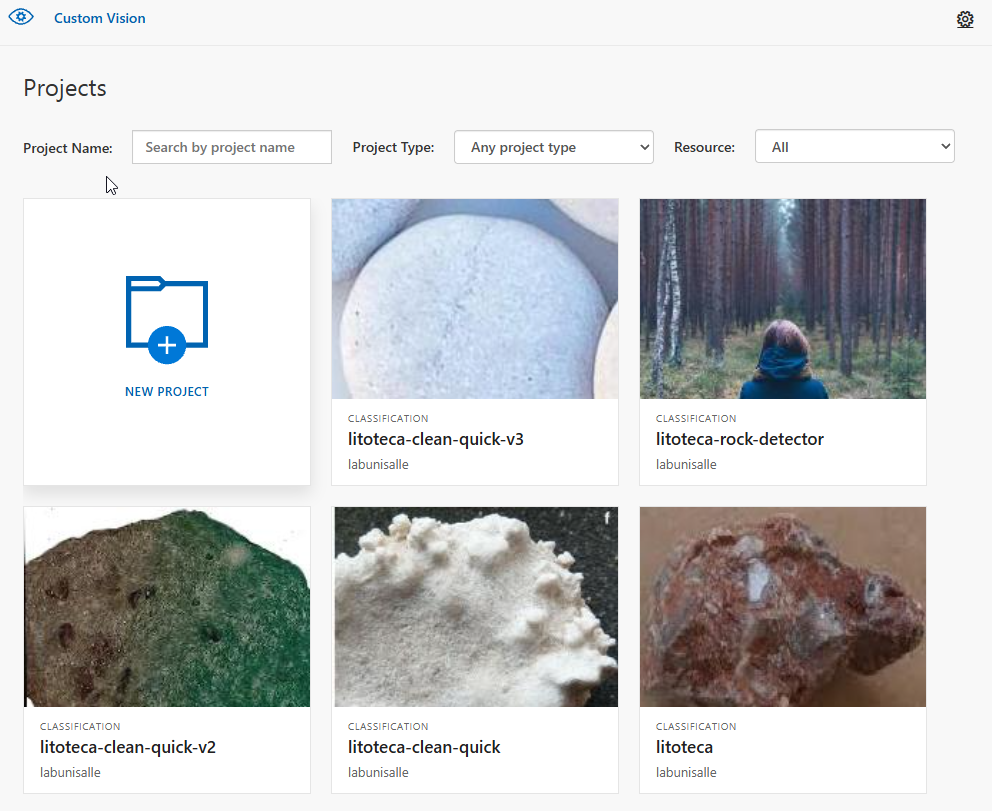
\includegraphics[width=0.95\linewidth]{assets/images/custom-vision-projects.png}
  \caption{Proyectos de Litoteca en Azure Custom Vision, incluyendo las iteraciones Quick y el detector roca/no-roca.}
  \label{fig:custom-vision}
\end{figure}

Se trabajaron tres iteraciones Quick completadas sobre el dataset limpio y una
iteración Advanced que terminó siendo la de mejor desempeño:

\begin{itemize}
  \item \textbf{Quick v1} (proyecto \texttt{litoteca-clean-quick}, iteración
        \texttt{6276ca2b-ad3e-4ca4-93ea-3be210b98771}): primera iteración
        completada, con validación API de 95/146 aciertos (65.07\%).
  \item \textbf{Quick v2} (proyecto \texttt{litoteca-clean-quick-v2}, iteración
        \texttt{4792fd31-2f7a-4505-9c72-71c1c3ffe4b8}): entrenamiento completado,
        publicado como \texttt{litoteca-v1} en \texttt{labunisalle-Prediction};
        luego fue reemplazado por la iteración Advanced publicada como
        \texttt{litoteca-v2}.
\end{itemize}

\begin{table}[H]
  \centering
  \caption{Comparación global entre iteraciones Quick completadas}
  \label{tab:metricas-globales}
  \begin{tabular}{@{}lrrr@{}}
    \toprule
    Iteración & Precision & Recall & AP \\
    \midrule
    Quick v1 (6276ca2b) & 83.08\% & 52.43\% & 72.74\% \\
    Quick v2 (4792fd31) & 84.88\% & 54.48\% & 77.77\% \\
    Quick v3 (9354cec6) & 79.70\% & 54.58\% & 74.64\% \\
    Advanced (d538f641) & 98.66\% & 96.22\% & 98.42\% \\
    \bottomrule
  \end{tabular}
\end{table}

La iteración Advanced mejora las métricas globales respecto a todas las Quick,
especialmente en recall y AP. El desempeño es alto y parejo en las nueve clases,
incluidas las que concentraban confusión en las iteraciones anteriores
(\emph{shale}, \emph{clay} y \emph{chert}).

\subsubsection{Quick v3 y decisión de cierre}

Se entrenó Quick v3 como iteración curada adicional (proyecto
\texttt{litoteca-clean-quick-v3}, \texttt{601da1f6-4fa9-47c0-9177-26284667cc56},
iteración \texttt{9354cec6-b49a-400e-9ce9-0c4230254fd9}, tipo \texttt{Quick}).
El dataset de entrenamiento partió de v2 y recuperó 131 imágenes de v1 en clases
débiles/confusas (\emph{chert}, \emph{clay}, \emph{conglomerate},
\emph{diatomite}, \emph{shale}, \emph{siliceous-sinter}), quedando en 1278 train,
193 valid y 144 test.

Quick v3 obtuvo P 79.70\%, R 54.58\% y AP 74.64\%, con validación sintética API
de 96/146 (65.75\%). Al no superar a Quick v2 (P 84.88\%, R 54.48\%, AP 77.77\%;
101/146, 69.18\%), no se promovió.

\subsubsection{Iteración Advanced y modelo final}

La iteración Advanced del proyecto \texttt{litoteca}
(\texttt{d15445ca-24b1-4bcc-aa80-244fb2b8fd6a}, iteración
\texttt{d538f641-63da-4db3-8827-fe2e1f91cee9}) terminó después de 410 minutos de
entrenamiento y superó ampliamente a las iteraciones Quick: P 98.66\%, R 96.22\% y
AP 98.42\%. En la validación sintética API obtuvo 109/146 (74.66\%), frente a
101/146 (69.18\%) de Quick v2. Por ese resultado se publicó como
\texttt{litoteca-v2} en \texttt{labunisalle-Prediction} y se conectó a la aplicación
como modelo final, manteniendo el mismo contrato de la API.

\begin{table}[H]
  \centering
  \caption{Métricas por clase de la iteración Advanced}
  \label{tab:metricas-clase}
  \begin{tabular}{@{}lrrr@{}}
    \toprule
    Clase & Precision & Recall & AP \\
    \midrule
    basalt & 97.53\% & 98.75\% & 98.72\% \\
    chert & 98.61\% & 93.42\% & 97.15\% \\
    clay & 100.00\% & 91.46\% & 96.78\% \\
    conglomerate & 100.00\% & 97.59\% & 98.87\% \\
    diatomite & 97.40\% & 97.40\% & 97.69\% \\
    gypsum & 98.59\% & 95.89\% & 99.89\% \\
    olivine-basalt & 100.00\% & 98.61\% & 100.00\% \\
    shale & 97.30\% & 97.30\% & 98.72\% \\
    siliceous-sinter & 98.55\% & 95.77\% & 98.51\% \\
    \bottomrule
  \end{tabular}
\end{table}

\subsubsection{Detector roca/no-roca}

Para reducir falsos positivos ante imágenes fuera de dominio, se entrenó un modelo
binario separado en Custom Vision con dos etiquetas: \texttt{rock} y
\texttt{not\_rock}. El dataset de detección (\texttt{data/rock-detector}) contiene
150 imágenes de roca y 150 imágenes no-roca. La iteración
\texttt{2d92f618-115e-4a73-a9ed-006002782c7c} del proyecto
\texttt{2dc1aedb-f66c-4fb1-abc5-54c253440052} se publicó como
\texttt{litoteca-detector-v1} en \texttt{labunisalle-Prediction}.

\begin{table}[H]
  \centering
  \caption{Métricas del detector roca/no-roca}
  \label{tab:detector-metricas}
  \begin{tabular}{@{}lrrr@{}}
    \toprule
    Etiqueta / Global & Precision & Recall & AP \\
    \midrule
    not\_rock & 100.00\% & 100.00\% & --- \\
    rock & 100.00\% & 96.70\% & --- \\
    \midrule
    \textbf{Global} & \textbf{100.00\%} & \textbf{98.28\%} & \textbf{99.97\%} \\
    \bottomrule
  \end{tabular}
\end{table}

La Function \texttt{functions/api/predict.js} consulta primero el detector. Si la
etiqueta superior es \texttt{not\_rock} o la probabilidad de \texttt{rock} es menor
que 0.5, la API responde con HTTP 422 y código \texttt{no\_es\_roca}; solo cuando la
imagen pasa este guardrail se invoca el clasificador multiclase. Las credenciales y
endpoints de predicción se manejan como variables de entorno en Cloudflare Pages,
incluidos \texttt{CUSTOM\_VISION\_DETECTOR\_PROJECT} y
\texttt{CUSTOM\_VISION\_DETECTOR\_ITERATION}.

\subsection{Desarrollo de la aplicación}

\subsubsection{Arquitectura}

La aplicación es un sitio estático sin build: HTML, CSS y JavaScript vanilla. La
predicción se consume mediante una Cloudflare Pages Function en
\texttt{functions/api/predict.js}, que valida la imagen, ejecuta primero el detector
roca/no-roca y, solo si la imagen pasa el guardrail, envía la solicitud al
clasificador multiclase de Custom Vision. La respuesta se normaliza al contrato de
Litoteca.

\begin{table}[H]
  \centering
  \caption{Componentes principales de la aplicación}
  \label{tab:componentes}
  \begin{tabular}{@{}p{3.8cm}p{8.6cm}@{}}
    \toprule
    Componente & Responsabilidad \\
    \midrule
    \texttt{index.html} & Estructura de vistas: inicio, cámara, resultado e historial. \\
    \texttt{assets/app.js} & Lógica de UI, cámara, subida, historial local y presentación de resultados. \\
    \texttt{assets/app.css} & Sistema visual editorial/papel. \\
    \texttt{assets/fichas.js} & Fichas curadas de las 9 clases. \\
    \texttt{assets/wiki.js} & Extractos cacheados de Wikipedia con atribución CC BY-SA. \\
    \texttt{functions/api/predict.js} & Proxy a Custom Vision, guardrail roca/no-roca, validación y contrato. \\
    \texttt{sw.js} & Service worker para caché de recursos estáticos y comportamiento sin conexión~\cite{w3cserviceworkers}. \\
    \texttt{scripts/gates.sh} & Gates deterministas, pruebas de contrato y smoke test de navegador. \\
    \bottomrule
  \end{tabular}
\end{table}

\subsubsection{Interfaz de usuario}

La interfaz se diseñó con enfoque móvil, accesible y educativo. Incluye:

\begin{itemize}
  \item Captura con cámara o carga de imagen.
  \item Vista de resultado con clase, confianza, margen y alternativas.
  \item Fichas con explicación: qué es, cómo se formó, gemelas y señales.
  \item Historial local en el navegador.
  \item Modo sin conexión para recursos ya cacheados; la predicción en línea se
        desactiva cuando no hay red.
\end{itemize}

\subsubsection{Generación de ilustraciones}

Para reforzar el valor pedagógico, se generaron ilustraciones del proceso geológico
de cada roca. Las ilustraciones se produjeron con \texttt{facet + ComfyUI}
(workflow \texttt{flux2-klein-4b}) a partir de una pieza reproducible
(\texttt{tools/procesos-geologicos.toml}). Luego se optimizaron a WebP/PNG y se les
agregaron etiquetas de texto manualmente, evitando texto sintético generado por el
modelo de imagen.

\begin{figure}[H]
  \centering
  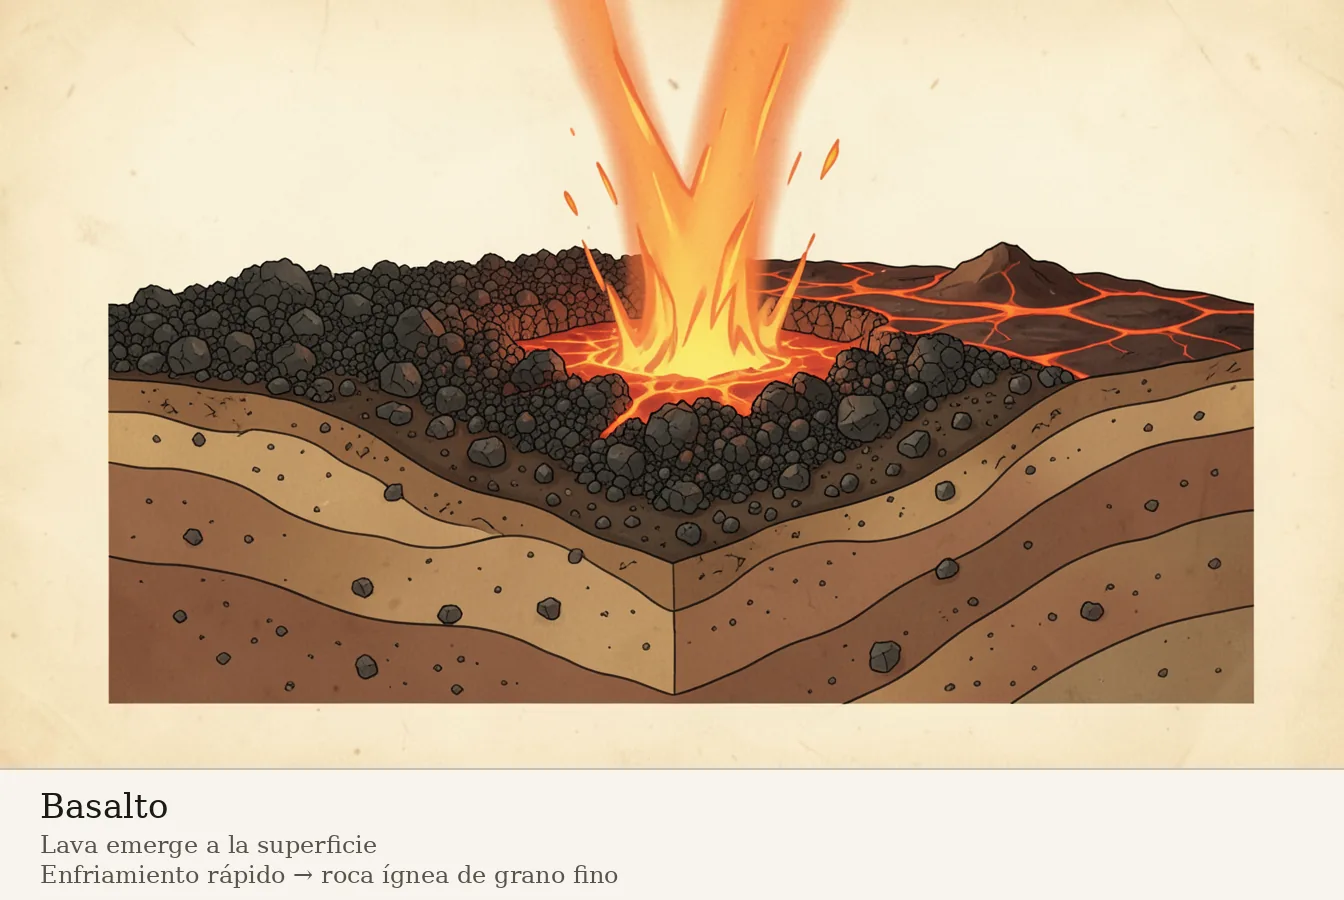
\includegraphics[width=0.82\linewidth]{assets/images/basalt.png}
  \caption{Ejemplo de ilustración generada para el proceso de formación del basalto}
  \label{fig:basalt}
\end{figure}

\subsection{Despliegue}

La aplicación se despliega en Cloudflare Pages~\cite{cloudflarepages}. El flujo de
despliegue usa GitHub Actions con \texttt{workflow\_dispatch} desde la rama
\texttt{develop}, entorno \texttt{production}, y \texttt{wrangler pages deploy}.
Los secretos de Cloudflare se configuran en GitHub Environment secrets; los secretos
de Custom Vision, incluidos los del detector roca/no-roca, se configuran en
Cloudflare Pages como variables de runtime de la Function.

La versión pública está disponible en \url{https://litoteca.pages.dev/}
\cite{litotecaapp}. La demo en video está disponible en
\url{https://youtu.be/X435kZhNOG8}.

  \section{Validación y resultados}
\label{sec:results}

\subsection{Resultados de preparación de datos}

La preparación del dataset permitió pasar de un export con fuga entre splits a un
conjunto trazable. Los principales resultados de esta etapa son:

\begin{itemize}
  \item 4.212 archivos originales analizados; 1.754 clusters/originales identificados.
  \item 55 descartes por duplicados o casi-duplicados en evaluación.
  \item 284 pares de casi-duplicados entre clusters y 22 conflictos de etiqueta
        documentados.
  \item Split limpio sin intersección de clusters: 3.428 train, 209 valid, 146 test.
  \item Versión limpia para entrenamiento: 1.325 train, 209 valid, 146 test, con una
        imagen por cluster y exclusión de conflictos de etiqueta.
\end{itemize}

La limpieza de conflictos es relevante porque varias confusiones esperadas ocurren
entre clases visualmente similares, en especial \emph{chert}, \emph{diatomite} y
\emph{siliceous-sinter} (geiserita). La Figura~\ref{fig:siliceas} ilustra ejemplos
de procesos asociados a estas clases.

\begin{figure}[H]
  \centering
  \begin{minipage}{0.48\linewidth}
    \centering
    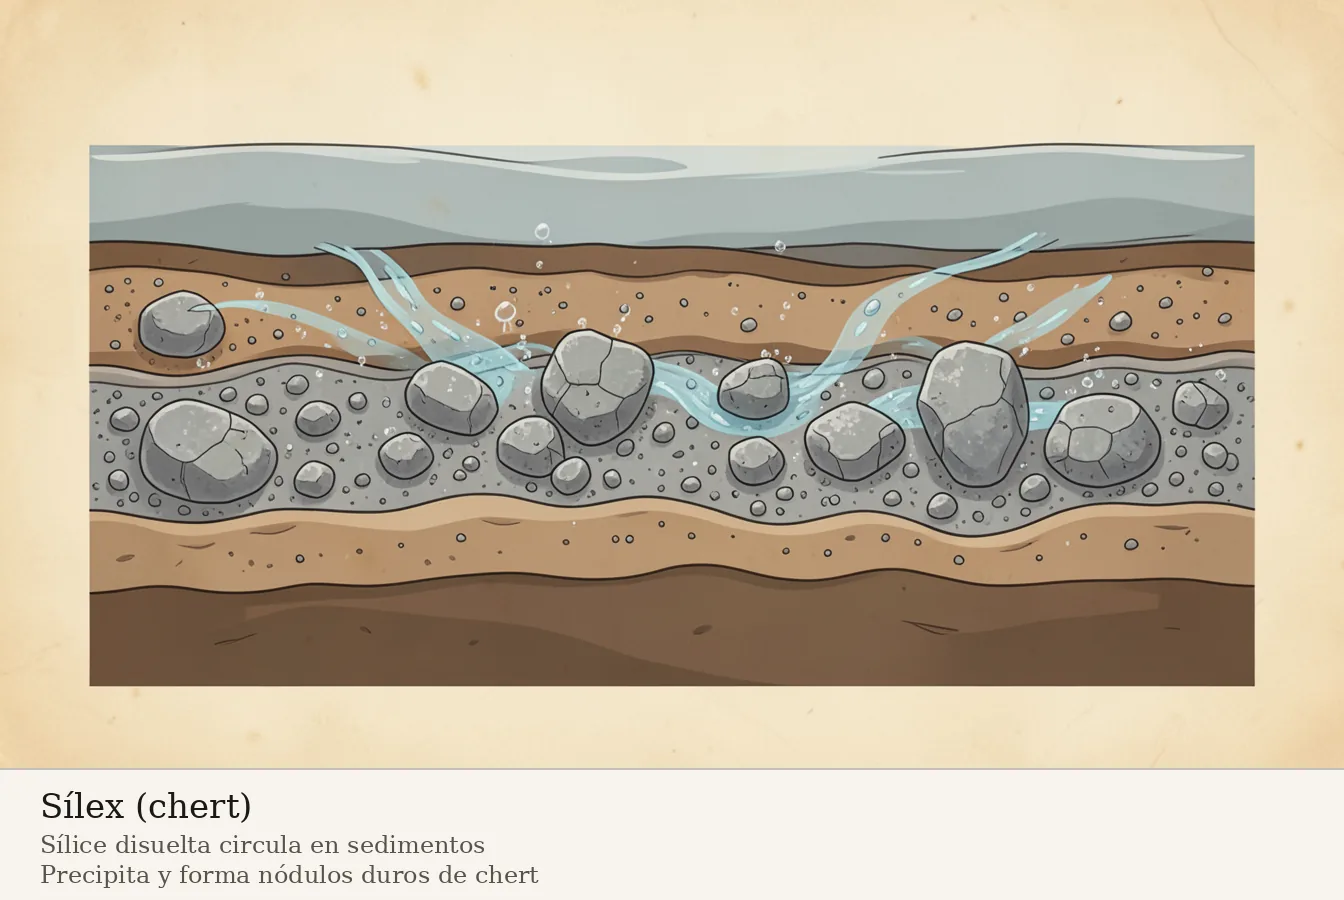
\includegraphics[width=\linewidth]{assets/images/chert.png}
  \end{minipage}\hfill
  \begin{minipage}{0.48\linewidth}
    \centering
    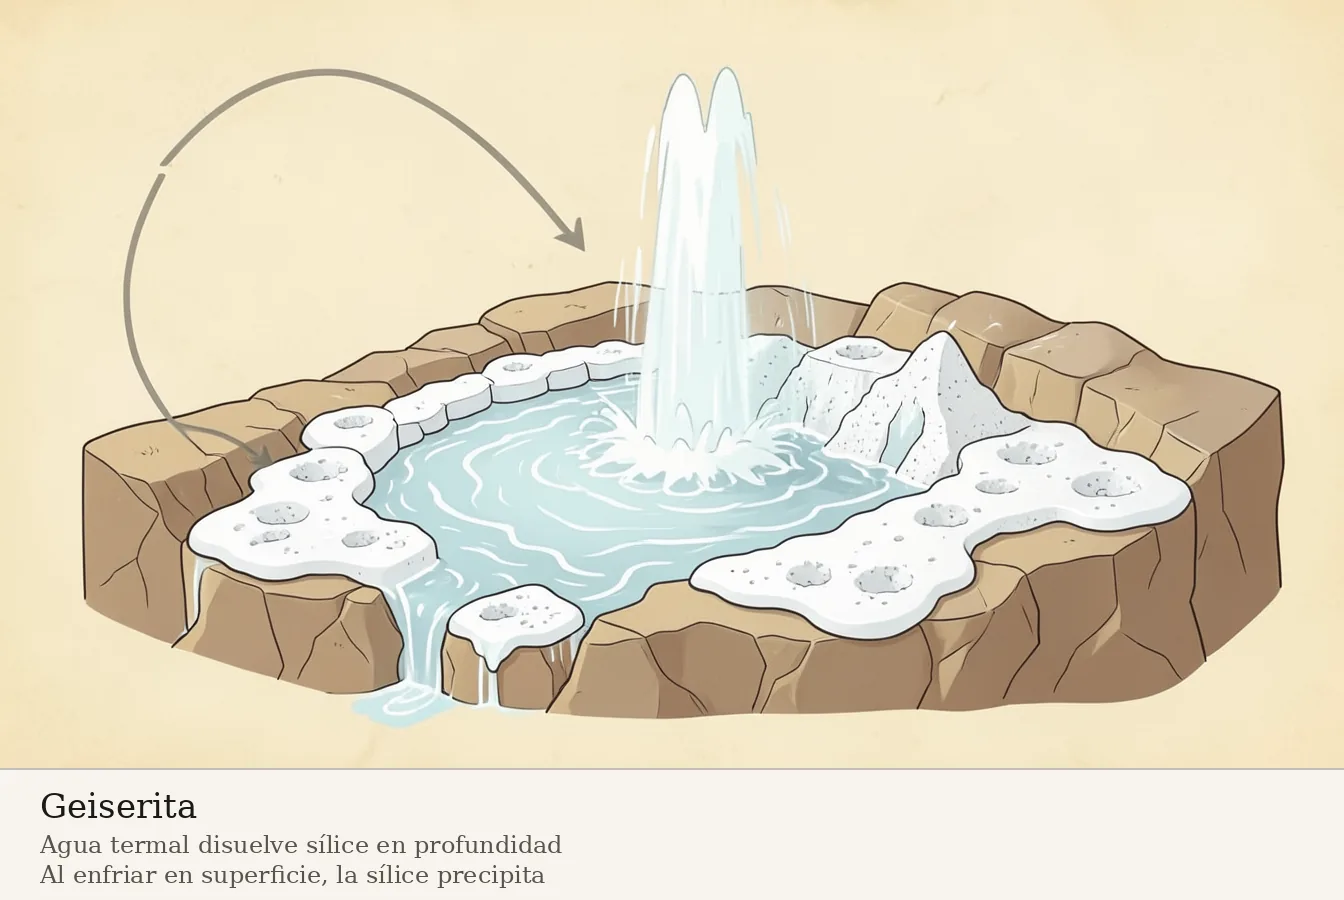
\includegraphics[width=\linewidth]{assets/images/siliceous-sinter.png}
  \end{minipage}
  \caption{Ejemplos de ilustraciones de proceso para clases síliceas}
  \label{fig:siliceas}
\end{figure}

\subsection{Estado de la aplicación}

La aplicación Litoteca se encuentra desplegada en Cloudflare Pages
\cite{litotecaapp}. El repositorio público está en GitHub \cite{litotecarepo}. La
Tabla~\ref{tab:funcionalidades} resume el estado de las funcionalidades relevantes
para la entrega.

\begin{table}[H]
  \centering
  \caption{Estado de funcionalidades implementadas}
  \label{tab:funcionalidades}
  \begin{tabular}{@{}p{4.3cm}p{8.1cm}@{}}
    \toprule
    Funcionalidad & Estado \\
    \midrule
    Carga/captura de imagen & Implementada, con validación de tipo y tamaño. \\
    Ficha por clase & Implementada para las 9 clases, con extractos cacheados de Wikipedia~\cite{wikipedia}. \\
    Historial local & Implementado con \texttt{localStorage}. \\
    Proxy de predicción & Implementado en \texttt{functions/api/predict.js}. \\
    Guardrail roca/no-roca & Implementado; el detector binario se consulta antes del clasificador y responde HTTP 422 con código \texttt{no\_es\_roca}. \\
    Modo sin conexión & Implementado con service worker y mensaje honesto para predicción en línea~\cite{w3cserviceworkers}. \\
    Despliegue CF Pages & Implementado con GitHub Actions y Wrangler. \\
    Modelo Advanced & Publicado como \texttt{litoteca-v2} y conectado como clasificador final (P 98.66\%, R 96.22\%, AP 98.42\%). \\
    Quick v3 evaluado & Completado (P 79.70\%, R 54.58\%, AP 74.64\%; validación API 96/146, 65.75\%); no superó a Quick v2, no se promovió. \\
    \bottomrule
  \end{tabular}
\end{table}

\begin{figure}[H]
  \centering
  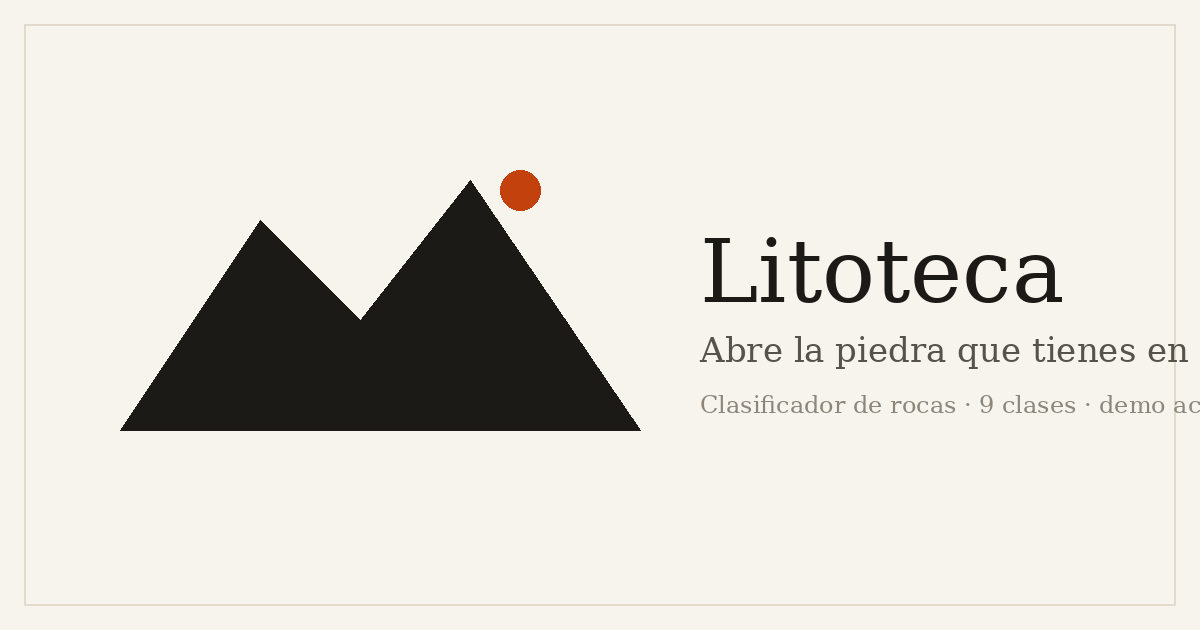
\includegraphics[width=0.75\linewidth]{assets/images/og-image.png}
  \caption{Vista de identidad visual de Litoteca}
  \label{fig:og}
\end{figure}

\subsection{Validación sintética por API}

Se ejecutó una validación sintética contra la iteración publicada actualmente como
\texttt{litoteca-v2} (Advanced, \texttt{d538f641-63da-4db3-8827-fe2e1f91cee9}) usando
el conjunto \texttt{data/prepared-clean-train/test} (146 imágenes, una por cluster,
sin fuga). La llamada se realizó al endpoint de predicción de Custom Vision con el
mismo contrato que consume la aplicación.

\begin{table}[H]
  \centering
  \caption{Validación sintética por API (test limpio, Advanced)}
  \label{tab:api-test}
  \begin{tabular}{@{}lrrr@{}}
    \toprule
    Clase & Aciertos & Total & Accuracy \\
    \midrule
    basalt & 14 & 15 & 93.33\% \\
    chert & 11 & 14 & 78.57\% \\
    clay & 6 & 12 & 50.00\% \\
    conglomerate & 9 & 13 & 69.23\% \\
    diatomite & 12 & 19 & 63.16\% \\
    gypsum & 19 & 23 & 82.61\% \\
    olivine-basalt & 18 & 19 & 94.74\% \\
    shale & 11 & 20 & 55.00\% \\
    siliceous-sinter & 9 & 11 & 81.82\% \\
    \midrule
    \textbf{Total} & \textbf{109} & \textbf{146} & \textbf{74.66\%} \\
    \bottomrule
  \end{tabular}
\end{table}

Frente a Quick v2 (101/146, 69.18\%), la iteración Advanced mejora en 8 aciertos
(+5.48 puntos porcentuales). Los errores remanentes se concentran en clases
visualmente cercanas: \emph{conglomerate}$\rightarrow$\emph{siliceous-sinter} (3),
\emph{diatomite}$\rightarrow$\emph{chert} (3),
\emph{shale}$\rightarrow$\emph{conglomerate} (3),
\emph{chert}$\rightarrow$\emph{diatomite} (2),
\emph{clay}$\rightarrow$\emph{shale} (2),
\emph{clay}$\rightarrow$\emph{siliceous-sinter} (2),
\emph{shale}$\rightarrow$\emph{chert} (2),
\emph{shale}$\rightarrow$\emph{diatomite} (2) y
\emph{siliceous-sinter}$\rightarrow$\emph{chert} (2). La mejora es consistente con
las métricas de entrenamiento y reduce la brecha entre validación y uso real.

  \section{Conclusiones}
\label{sec:conclusions}

Litoteca integra un flujo completo de clasificación de rocas en una aplicación web
móvil: preparación trazable del dataset, entrenamiento en Azure Custom Vision, proxy
de predicción en Cloudflare Pages y una interfaz que presenta la predicción con
contexto geológico. El aporte principal no es solo la etiqueta de clase, sino la
combinación de clasificación, guardrail roca/no-roca y ficha explicativa para un
usuario no experto.

La preparación de datos fue decisiva para la credibilidad del modelo. La
deduplicación por imagen original, la reconstrucción de splits sin fuga y la
exclusión de conflictos de etiqueta redujeron el riesgo de métricas optimistas. Los
resultados verificados de Quick v2 y del detector roca/no-roca muestran un prototipo
funcional, con buen desempeño en varias clases y confusiones concentradas en
familias visualmente cercanas.

Como limitaciones actuales, el prototipo cubre nueve clases ígneas y sedimentarias,
depende de la calidad de la fotografía y del endpoint de predicción, y mantiene
recall bajo en clases difíciles como \emph{shale}, \emph{clay} y \emph{chert}. La
validación sintética por API aporta evidencia reproducible, pero no sustituye una
evaluación de campo más amplia.

El documento se cierra con Quick v3 evaluado: obtuvo P 79.70\%, R 54.58\% y AP
74.64\%, con validación sintética API de 96/146 (65.75\%), sin superar a Quick v2.
Por ello, la entrega se mantiene con Quick v2 como modelo publicado. El
entrenamiento Advanced permanece como trabajo futuro: si completa y mejora el
desempeño verificado, podrá conectarse por debajo del mismo contrato de la
aplicación sin cambiar la experiencia de usuario.


  \clearpage
  \phantomsection
  \addcontentsline{toc}{section}{\refname}
  \bibliographystyle{plain}
  \bibliography{bib/references}

  \appendix
  \section{Material suplementario}
\label{app:supplementary}

\subsection{Enlaces del proyecto}

\begin{table}[H]
  \centering
  \caption{Recursos del proyecto Litoteca}
  \label{tab:recursos}
  \begin{tabular}{@{}p{4.2cm}p{8.2cm}@{}}
    \toprule
    Recurso & URL / referencia \\
    \midrule
    Repositorio GitHub & \url{https://github.com/JheisonMB/litoteca} \\
    Aplicación desplegada & \url{https://litoteca.pages.dev/} \\
    Demo en video & \url{https://youtu.be/X435kZhNOG8} \\
    Dataset fuente & \url{https://www.kaggle.com/datasets/stealthtechnologies/rock-classification} \\
    Azure Custom Vision & \url{https://learn.microsoft.com/azure/ai-services/custom-vision-service/overview} \\
    \bottomrule
  \end{tabular}
\end{table}

\subsection{Trazabilidad del dataset}

El dataset preparado incluye los siguientes artefactos en \texttt{data/prepared/}:

\begin{itemize}
  \item \texttt{manifest.csv}: procedencia, split, clase, hash perceptual.
  \item \texttt{stats.json}: conteos por clase y motivos de descarte.
  \item \texttt{conflicts.csv}: pares con etiqueta contradictoria.
  \item \texttt{near\_duplicates.csv}: casi-duplicados entre clusters.
  \item \texttt{descartadas.csv}: registros excluidos.
\end{itemize}

Para el entrenamiento limpio se generó \texttt{data/prepared-clean-train/} con una
imagen por cluster y exclusión de conflictos de etiqueta. El reporte de limpieza se
encuentra en \texttt{clean\_report.json}.

\subsection{Variables de runtime de la Function}

El despliegue se realiza con GitHub Actions (\texttt{.github/workflows/deploy.yml})
y Cloudflare Wrangler. Los secretos del modelo se configuran en Cloudflare Pages
como variables de runtime de la Function, no en el frontend:

\begin{itemize}
  \item \texttt{CUSTOM\_VISION\_ENDPOINT}
  \item \texttt{CUSTOM\_VISION\_KEY}
  \item \texttt{CUSTOM\_VISION\_PROJECT}
  \item \texttt{CUSTOM\_VISION\_ITERATION}
  \item \texttt{CUSTOM\_VISION\_DETECTOR\_PROJECT}
  \item \texttt{CUSTOM\_VISION\_DETECTOR\_ITERATION}
  \item \texttt{CUSTOM\_VISION\_TRAINED} (opcional, metadato de despliegue)
\end{itemize}


\end{document}
